\documentclass[12pt,a4paper]{ctexart}

% ==== 页面设置 ====
\usepackage[top=2cm, bottom=2cm, left=2.2cm, right=2.2cm]{geometry}
\usepackage{amsmath, amssymb, amsthm}
\usepackage{enumitem}
\usepackage{multicol}
\usepackage{booktabs}
\usepackage{titlesec}
\usepackage{fancyhdr}
\usepackage{hyperref}
\usepackage{bm}
\usepackage{xcolor}
\usepackage{tikz}
\usetikzlibrary{arrows.meta, automata, positioning, bending}

\setlength{\headheight}{14pt}

% ==== 页眉页脚 ====
\pagestyle{fancy}
\fancyhf{}
\fancyhead[L]{\small 信息论 · 2026 春期末考试（回忆版）}
\fancyfoot[C]{\thepage}
\renewcommand{\headrulewidth}{0.4pt}

\newcommand{\EE}{\mathbb{E}}
\newcommand{\PP}{\mathbb{P}}
\newcommand{\XX}{\mathcal{X}}
\newcommand{\YY}{\mathcal{Y}}
\newcommand{\DKL}{D_{\mathrm{KL}}}
\newcommand{\indep}{\perp\!\!\!\perp}
\newcommand{\iid}{\overset{\text{i.i.d.}}{\sim}}

\begin{document}

\begin{center}
{\Huge\heiti 信息论 · 2026 年春季期末考试}\\[3mm]
{\Large\heiti （回忆版）}\\[2mm]
{\small 注：题目表述可能与原卷有出入，考点和数值已尽力还原。选择题共 10 题，有 1 题实在印象不太清楚（很简单），回忆不起来。}
\end{center}

\vspace{4mm}

% ============================================================
\section*{第一部分：客观题}

\vspace{-6mm}

\subsection*{一、单项选择题（共 9 小题）}

\begin{enumerate}[label=\arabic*., leftmargin=*]

\item 下列哪一项\textbf{不属于}信息论的理论框架？
\begin{multicols}{2}
\begin{enumerate}[label=(\Alph*)]
  \item 调制与解调
  \item 信源编码
  \item 噪声信道编码
  \item 率失真理论
\end{enumerate}
\end{multicols}

\item 由 KL 散度的非负性 $\DKL(p\|q) \geq 0$ 可以直接推出以下哪些结论？
\begin{enumerate}[label=(\Alph*)]
  \item 互信息 $I(X;Y) \geq 0$
  \item 条件熵 $H(X|Y) \leq H(X)$
  \item 均匀分布的熵最大：$H(p) \leq \log|\XX|$
  \item 以上都对
\end{enumerate}

\item 关于 AEP 和信源定长编码定理，以下说法\textbf{正确}的是：
\begin{enumerate}[label=(\Alph*)]
  \item 当 $n\to\infty$ 时，非典型序列的出现概率趋近于零
  \item 典型集的大小严格等于 $2^{nH(X)}$
  \item 信源定长编码所需的比特数约为 $n\log|\XX|$
  \item 典型集中每个序列的概率相等
\end{enumerate}

\item 关于 Huffman 编码，以下说法\textbf{错误}的是：
\begin{enumerate}[label=(\Alph*)]
  \item Huffman 码的码长满足 Kraft 不等式
  \item 平均码长 $L$ 满足 $H(X) \leq L < H(X)+1$
  \item Huffman 码的码长取 $l(x) = -\lceil\log p(x)\rceil$
  \item Huffman 码在所有唯一可译码中平均码长最短
\end{enumerate}

\item 关于 Hamming 码的性质，以下说法\textbf{错误}的是：
\begin{enumerate}[label=(\Alph*)]
  \item Hamming 码可检测一位或两位错误
  \item Hamming 码可纠正一位错误
  \item 不同码字之间的最小 Hamming 距离 $\geq 3$
  \item Hamming 距离是奇偶校验的基础
\end{enumerate}

\item 关于信道编码定理，以下说法\textbf{错误}的是：
\begin{enumerate}[label=(\Alph*)]
  \item 若 $R < C$，存在编码方案使 $P_e \to 0$
  \item 若 $R > C$，任何编码方案都有 $P_e > 0$
  \item 信道容量 $C = \max_{P_X} I(X;Y)$
  \item 反馈可以增加离散无记忆信道的信道容量
\end{enumerate}

\item 关于率失真函数 $R(D)$ 的性质，以下说法\textbf{错误}的是：
\begin{enumerate}[label=(\Alph*)]
  \item $R(D)$ 是 $D$ 的单调非增函数
  \item $R(D)$ 是 $D$ 的凸函数
  \item $R(0) = H(X)$
  \item $R(D)$ 曲线与 $x$ 轴交于无穷远
\end{enumerate}

\item 联合典型引理（JTL）在以下哪个定理的证明中\textbf{未}被使用？
\begin{multicols}{2}
\begin{enumerate}[label=(\Alph*)]
  \item 噪声信道编码定理
  \item 率失真定理
  \item 信源定长编码定理
  \item 以上都使用了 JTL
\end{enumerate}
\end{multicols}

\item 信息论除了应用于通信领域，还可应用于：
\begin{enumerate}[label=(\Alph*)]
  \item 压缩感知（Compressed Sensing）
  \item 变分自编码器（VAE）
  \item 投资组合优化
  \item 以上都对
\end{enumerate}

\end{enumerate}

\subsection*{二、判断题（共 10 小题）\\
（正确打``$\surd$''，错误打``$\times$''）}

\begin{enumerate}[label=\arabic*., leftmargin=*]

\item 熵 $H(p)$ 关于概率分布 $p$ 是凹函数。 \hfill（\quad）

\item 互信息 $I(X;Y)$ 可以描述变量之间的非线性相关关系。 \hfill（\quad）

\item 在信源定长编码定理的证明中，独立同分布假设过强，在实际中没有应用价值。 \hfill（\quad）

\item 均匀分布的信息熵最大，因此均匀分布的数据不可压缩。 \hfill（\quad）

\item 在不可约马尔可夫链中，若状态转移矩阵存在自环（对角元 $>0$），则该链是非周期的。 \hfill（\quad）

\item 给定方差约束，高斯分布使微分熵最大。 \hfill（\quad）

\item 无功率约束的高斯信道仍具有实际应用价值。 \hfill（\quad）

\item 由 Kraft-McMillan 定理可知，只考虑前缀码是不损失最优性的。 \hfill（\quad）

\item Huffman 码的所有码字长度都严格小于其他前缀码的对应码字长度。 \hfill（\quad）

\item 在平稳遍历信源和离散无记忆信道中，信源信道分离编码方案在所有可达方案中是最优的，联合编码不能超越。 \hfill（\quad）

\end{enumerate}

% ============================================================
\section*{第二部分：解答题}

\subsection*{三、Hamming 码}

给定 Hamming 矩阵：
\setcounter{MaxMatrixCols}{15}
{\small
\[
H = \begin{bmatrix}
0&0&0&0&0&0&0&1&1&1&1&1&1&1&1\\
0&0&0&1&1&1&1&0&0&0&0&1&1&1&1\\
0&1&1&0&0&1&1&0&0&1&1&0&0&1&1\\
1&0&1&0&1&0&1&0&1&0&1&0&1&0&1
\end{bmatrix}
\]
}

\begin{enumerate}[label=(\arabic*), nosep]
  \item 求码长 $n$ 和 $m$，并求可编码的数据位数；
  \item 指出哪些位是数据位，并写出校验位 $x_1, x_2, x_4, x_8$ 各自负责校验的数据位；
  \item 接收端收到以下两个 15 bit 的接收序列，判断是否有误；如有误，假设至多一位出错，指出错误位并纠正。
  \begin{enumerate}
    \item $y_a = (0,0,1,0,1,0,0,1,1,0,1,1,0,1,1)^T$
    \item $y_b = (1,0,1,1,0,1,0,0,1,1,0,1,1,0,1)^T$
  \end{enumerate}
  \item 证明：该 Hamming 码的码字空间中，任意两个不同码字的 Hamming 距离 $\geq 3$。
\end{enumerate}

\subsection*{四、高斯信道与充分统计量}

\begin{enumerate}[label=(\arabic*), nosep]
  \item 设 $X_1,\ldots,X_n \iid \mathcal{N}(\mu, \sigma^2)$，$\mu$ 和 $\sigma^2$ 均未知。\\
  写出参数 $(\mu, \sigma^2)$ 的充分统计量，并说明理由。

  \item 在推导高斯信道容量时，为什么必须考虑功率约束？

  \item 五个并行高斯子信道，噪声功率分别为：
  \[
  N_1=1,\; N_2=4,\; N_3=2,\; N_4=6,\; N_5=8
  \]
  总功率约束 $P = 15$。利用水填充算法求最优功率分配 $P_1^*, P_2^*, P_3^*, P_4^*, P_5^*$；

\end{enumerate}

\subsection*{五、平稳马尔可夫链}

某平稳马尔可夫链的状态转移图如下所示（课件 Lecture 6 原题）：

\begin{center}
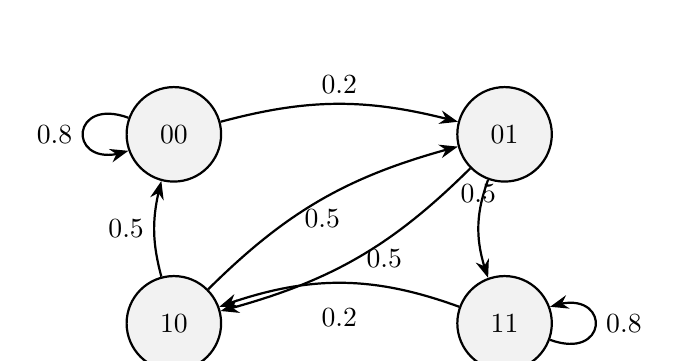
\begin{tikzpicture}[>=Stealth, scale=1.2]
  % Node positions
  \node[circle, draw, thick, fill=gray!10, minimum size=12mm] (S1) at (0,2)   {$00$};
  \node[circle, draw, thick, fill=gray!10, minimum size=12mm] (S2) at (3.5,2) {$01$};
  \node[circle, draw, thick, fill=gray!10, minimum size=12mm] (S3) at (0,0)   {$10$};
  \node[circle, draw, thick, fill=gray!10, minimum size=12mm] (S4) at (3.5,0) {$11$};

  % Self-loops (arcs)
  \draw[->, thick] (S1) .. controls ++(160:1.2) and ++(200:1.2) .. (S1)
        node[pos=0.5, left] {0.8};
  \draw[->, thick] (S4) .. controls ++(-20:1.2) and ++(20:1.2) .. (S4)
        node[pos=0.5, right] {0.8};

  % Transitions
  \draw[->, thick] (S1) to[bend left=15] node[above] {0.2} (S2);
  \draw[->, thick] (S2) to[bend left=15] node[right] {0.5} (S3);
  \draw[->, thick] (S2) to[bend right=20] node[above=2mm] {0.5} (S4);
  \draw[->, thick] (S3) to[bend left=15] node[left] {0.5} (S1);
  \draw[->, thick] (S3) to[bend left=15] node[below] {0.5} (S2);
  \draw[->, thick] (S4) to[bend right=20] node[below=2mm] {0.2} (S3);

\end{tikzpicture}
\end{center}

\begin{enumerate}[label=(\arabic*), nosep]
  \item 什么是平稳马尔可夫过程？为什么平稳马尔可夫信源可以用状态转移矩阵来描述？

  \item 写出该马尔可夫链的状态转移矩阵 $P$，标明各状态对应的行/列。

  \item 求该链的稳态分布，并计算熵率。

  \item 判断该链是否是遍历的（ergodic），说明理由。
\end{enumerate}

\subsection*{六、噪声信道编码定理}

\begin{enumerate}[label=(\arabic*), nosep]
  \item 解释以下符号的定义：$R$、$M$、$n$、$C_I$。

  \item 说明 $H(Y|X)$ 和 $H(X|Y)$ 在通信系统中的物理含义。

  \item 写出噪声信道编码定理\textbf{正向证明}（若 $R < C$ 则存在编码方案使 $P_e \to 0$）的关键步骤。\\
  包括：随机码本如何构造、译码策略、误差如何分析和放缩、如何得到结论。

  \item 写出\textbf{反向证明}（若 $R > C$ 则任何编码方案都有 $P_e > 0$）的关键步骤，\\
  列出用到的主要不等式及其作用。说明为什么不假设 $X^n, Y^n$ 独立同分布。

  \item 用几何语言解释噪声信道编码定理。
\end{enumerate}

\end{document}
